\section{Versuchsaufbau}
Der Versuch ist aus vier Grundbausteinen aufgebaut die in Abbildung \ref{fig:versuchsaufbau}
gezeigt sind. Dabei bilden ein Permanentmagnet, ein digitales Speicheroszilloskop sowie ein
PS2-Controller und ein Steuermodul die Hauptbestandteile.
\begin{figure}
    \center
    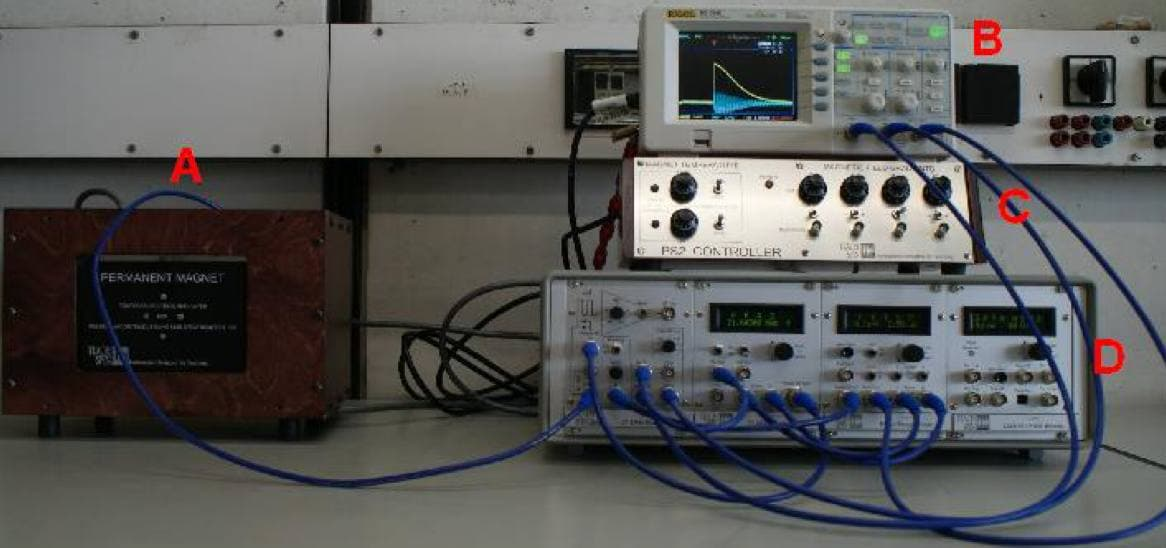
\includegraphics[width=0.8\textwidth]{bilder/versuchsaufbau.jpg}
    \caption{Dargestellt ist der Versuchsaufbau mit einem Permanentmagneten A, einem digitales Speicheroszilloskop B, einem
    PS2-Controller C und einem Steuermodul D\cite{anleitung}}
    \label{fig:versuchsaufbau}
\end{figure}

\subsection{Grundeinstellungen der Apperatur}
\subsubsection*{21 MHz Synthesizer}
Damit lässt sich die Frequenz-Veränderung des rf-Impulses variieren. Diese wird für die folgende
Versuchsreihe auf ca. $21,6\,$MHz eingestellt.
\subsubsection*{Impuls Programmierer}
Der Impuls kann darüber hinaus mit dem Programmierungs-Baustein weiter modifziert werden.
Dabei kann die Länge der jeweiligen Impulse sowie die Anzahl und Wiederholzeit der Impulssequenz eingestellt werden.
Die Wiederholzeit $P$ wird dabei auf ca. $800\,$ms eingestellt. $P$ muss dabei deutlich größer als die Relaxationszeit der Probe sein,
sodass sich das Spin-System wieder vollständig berruhigen kann.
\subsubsection*{Permanentmagnet und Controller}
Der Magnet liefert ein temperaturabhängiges Magnetfeld von $0,5\,$T. Des weiteren verfügt er 
über eine Temperaturreglung um die Temperatur und somit das Magnetfeld konstant zu halten. 
Über die LED-Anzeige wird der Temperatursollwert so eingestellt, das die LEDs nicht mehr leuchten.\\
Über die vier enthaltenen Spulen lässt sich ein 
Feldjeweils linear in x-, y-y und z-Richtung aufbauen. Die vierte Spule ermöglicht eine Erzeugung eines Feldgradientens
in $z^2$-Richtung. Somit ist eine Erzeugung eines homogenen Feldes sowie Feinjustierung einzelner Feldgradienten möglich.

\subsection{Grundparameter justieren}
Zunächst wird ein Proberöhrchen aus Wasser mit Kupfersulfat in das justierete homogene Magnetfeld gestellt. Dabei sorgt das Kupfersulfat dafür,
dass die Relaxionszeit vom Wasser durch das zusätzliche große magnetische Moment der paramagnetischen Kupferionen abgesenkt wird.
Die Phase wird so eingestellt, dass der Realteil maximiert und der Imaginärteil möglichst verschwindet.
Ein $90°$-Impuls wird eingestellt und die exakte Lamorfrequenz des hochfrequenz Wechselfeldes, so eingestellt dass die Amplitude des FID am Oszilloskop maximal wird.
Bei richtiger Justage der x-, y-, z, $z^2$-Potentiometer wird eine einhüllende Exponentialfunktion des FID (Free induction Decay) mit langer Zerfallszeit deutlich.
Nach dem Einstellen des $180°$-Impulses verschwinden beide Graphen auf dem Oszilloskop vollständig.\\
Nun ist das Magnetfeld sowie die Frequenz optimal justiert.

\subsection{Relaxationszeiten-Messung}
Für die Messung der Relaxionszeit $T_1$ (Spin-Gitter) wird der A- bzw. B-Puls mit der zuvor bestimmten
Pulslänge eingestellt. Für jeden Pulsabstand $\tau$ wird die Amplitude des FID vermessen.
Dabei wird der Pulsabstand von $0,0001$ bis $2\,$s varriert, die Periode $P$ wird wie folgt eingestellt.
\begin{align*}
    \tau \leq \SI{1}{s} &\rightarrow P= \SI{10}{s}\\
    \tau > \SI{1}{s} &\rightarrow P= \SI{10}{s} +\tau
\end{align*} 
\newline

Für die Messung der Relaxationszeit $T_2$ (Spin-Gitter) wird der A-Puls auf die Pulslänge für einen $90°$-Puls eingestellt und der B-Puls
entsprechend dem $180°$-Puls. Für die Anzahl $N$ der Puls wird $N=100$ gewählt. Damit das System wieder in den Gleichgewichtszustand
zurückkehren kann wird für die Periode $P$ ein vielfaches von $T_1$ gewählt.
Die Messung des Oszilloskop werden jeweils einmal phasengleich und gegenphasig für die Pulse gespeichert.

\subsection{Diffusionsmessung}
Hierbei wird nun die Anzahl der Pulslänge wieder auf $N=1$ reduziert. Nach der Vergrößerung von $\tau$
wird nun die Höhe des Echomaximums vermessen, sowie die Temperatur der Spulen notiert.
\section{Durchführung}
\label{sec:Durchfuehrung}
